\documentclass[a4paper,12pt]{article}
\usepackage[english,ukrainian,russian]{babel}
\linespread{1}
\usepackage{ucs}
\usepackage[utf8]{inputenc}
\usepackage[T2A]{fontenc}
\usepackage[paper=portrait,pagesize]{typearea}
\usepackage{amsmath}
\usepackage{bigints}
\usepackage{amsfonts}
\usepackage{graphicx}
\usepackage{amssymb}
\usepackage{cancel}
\usepackage{gensymb}
\usepackage{multirow}
\usepackage{rotate} 
\usepackage{pdflscape}
\usepackage{bigstrut}
\usepackage[pageanchor]{hyperref}
\usepackage{chngpage}
\usepackage{fancybox,fancyhdr}
\newcommand\tab[1][1cm]{\hspace*{#1}}
\newcommand{\RomanNumeralCaps}[1]{\MakeUppercase{\romannumeral #1}}
\usepackage[left=20mm, top=20mm, right=15mm, bottom=15mm, nofoot]{geometry}


\begin{document}
    \pagestyle{fancy}
    \fancyhead{}
    \fancyhead[R]{ФІ-12 Завалій Олександр}
    \begin{center}
        \large{\textbf{Міністерство освіти і науки України\\
                Національний технічний університет України\\
                «Київський політехнічний інститут імені Ігоря Сікорського»\\
                Навчально-науковий Фізико-технічний інститут}}\\
        \hfill \break \hfill \break \hfill\break \hfill \break \hfill \break \hfill \break \hfill \break
        \hfill \break \hfill \break \hfill \break
        \begin{center}
            \normalsize{\textbf{ОПЕРАЦІЙНІ СИСТЕМИ\\
            Комп’ютерний практикум\\
            Робота №9}}
        \end{center}
    \end{center}
    \hfill \break \hfill \break \hfill \break \hfill \break \hfill \break \hfill \break \hfill \break
    \hfill \break \hfill \break \hfill \break \hfill \break 
    \begin{flushright}
        \large{ \hspace{35pt} Виконав:\\
            студент групи ФI-12\\
            Завалій Олександр\\} 
        \large{ \hspace{35pt} Перевірив:\\
        Кірієнко О.В.} 
    \end{flushright}
    \hfill \break \hfill \break \hfill \break \hfill \break \hfill \break \hfill \break \hfill \break
    \hfill \break
    \begin{center} \textbf{Київ-2023} \end{center}
    \thispagestyle{empty}

\newpage
    \begin{center}
        \section*{\bfseries{Робота №9.\\
        Засоби синхронізації і взаємодії процесів }}
    \end{center}
    \textbf{Мета:} \\
    \hangindent=1.5cm 
    \hangafter=+1 \noindent
    Оволодіння практичними навичками використання засобів міжпроцесової взаємодії в Linux. \\
    \begin{center}
        \Large{Варіант №5}
    \end{center}
    Зміст індивідуального завдання:

    Програма моделює роботу примітивної СКБД, що зберігає єдину таблицю в оперативній пам'яті. Виконуючи деякі цикли
    робіт, K породжених процесів за допомогою черги повідомлень передають батьківському процесові номер рядка і вміст, на
    який потрібно замінити дані, що у ньому зберігаються. Батьківський процес виконує зазначену операцію і повертає
    попередній вміст рядка, що був змінений.
    \begin{figure}[h!]
        \begin{minipage}[h]{1\linewidth}
            \centering
            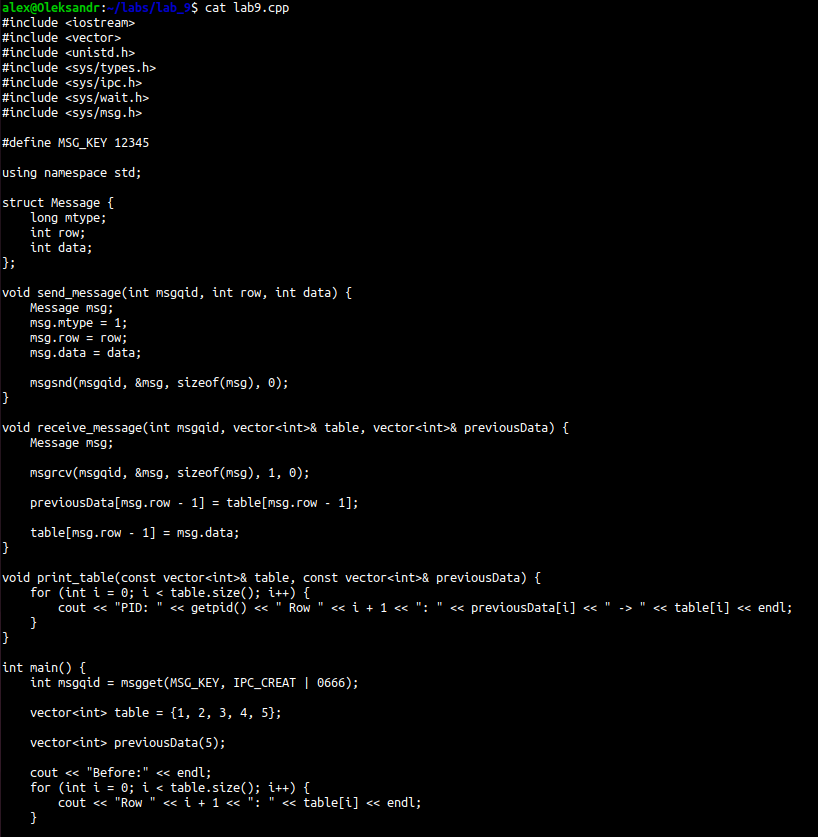
\includegraphics[width=0.8\linewidth]{Prt sc/Figure_1_1.png}  
        \end{minipage}
    \end{figure}

\newpage
    \begin{figure}[h!]
        \begin{minipage}[h]{1\linewidth}
            \centering
            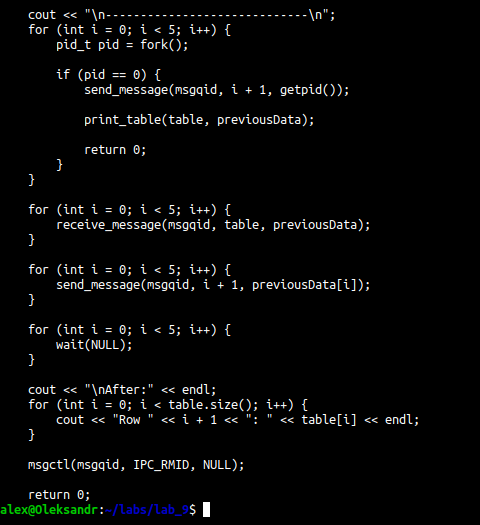
\includegraphics[width=0.8\linewidth]{Prt sc/Figure_1_2.png}  
        \end{minipage}
    \end{figure}

\newpage
    \begin{figure}[h!]
        \begin{minipage}[h]{1\linewidth}
            \centering
            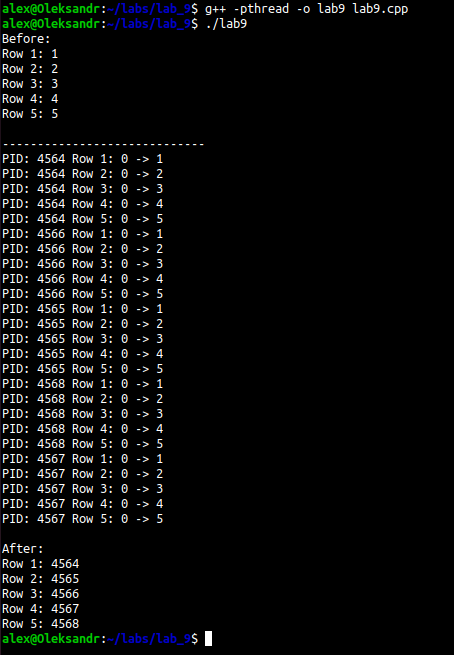
\includegraphics[width=0.8\linewidth]{Prt sc/Figure_2.png}  
        \end{minipage}
    \end{figure}

\newpage
    \begin{center}
        \Large{Висновки}
    \end{center}

    Міжпроцесна взаємодія (IPC) є важливою концепцією і має велике значення для розробки програм. 
    У контексті програмування існує кілька методів для здійснення IPC, кожен з яких має свої переваги та обмеження.

    Один із способів це використання черг повідомлень (Message Queues). Черги повідомлень дозволяють процесам обмінюватись даними шляхом надсилання повідомлень до черги. 
    З цієї ж черги інші процеси можуть повідомлення отримати. Цей метод забезпечує асинхронну комунікацію і може бути корисним у випадках, коли потрібно передавати 
    невеликі об'єкти даних між процесами.

    Ще один метод IPC це спільна пам'ять (Shared Memory). Використовуючи спільну пам'ять, кілька процесів можуть отримувати доступ до одного й того ж блоку пам'яті.
    Це дозволяє процесам ефективно обмінюватися великими об'єктами даних, не потребуючи копіювання даних між процесами. 
    Однак, спільна пам'ять вимагає синхронізації для уникнення конфліктів доступу до спільних ресурсів.

    Також, у Linux існує можливість використання сокетів (Sockets) для забезпечення мережевої взаємодії між процесами, які працюють на різних вузлах мережі.
    Сокети дозволяють передавати дані через мережу, використовуючи різні протоколи, такі як TCP або UDP.

    При розробці програм, які мають взаємодію між процесами, важливо враховувати характеристики і обмеження кожного методу IPC, а також забезпечити відповідну 
    синхронізацію для надійної і безпечної взаємодії між процесами.

\end{document}